\chapter{App Development}

\thispagestyle{empty}



\section{Backend}
\begin{itemize}
	\item \textbf{Framework:} FastAPI
	\begin{itemize}
		\item \textbf{Definition:} FastAPI is a modern web framework for building APIs with Python 3.6+ based on standard Python type hints. It is designed to be easy to use and efficient, making it a popular choice for building APIs.
		\item \textbf{Features:} FastAPI provides automatic generation of interactive API documentation using Swagger UI and ReDoc, input validation, dependency injection, and support for asynchronous programming with Python's \texttt{async} and \texttt{await} keywords.
	\end{itemize}
	\item \textbf{Dependencies:}
	\begin{itemize}
		\item \textbf{uvicorn:} Uvicorn is a lightning-fast ASGI server implementation, using uvloop and httptools. It is the recommended server for running FastAPI applications.
		\item \textbf{joblib:} Joblib is a set of tools to provide lightweight pipelining in Python. It is particularly useful for creating and persisting machine learning models.
	\end{itemize}
	\item \textbf{Endpoints:}
	\begin{itemize}
		\item \textbf{GET "/":} Returns a welcome message.
		\item \textbf{POST "/detect":} Accepts a pcap traffic file, extracts features, performs traffic classification using a pre-trained machine learning model, and returns the analysis results.
	\end{itemize}
\end{itemize}

\section{Frontend}
\begin{itemize}
	\item \textbf{Framework:} Vue.js
	\begin{itemize}
		\item \textbf{Definition:} Vue.js is a progressive JavaScript framework used for building user interfaces. It is designed to be incrementally adoptable and can be easily integrated into other projects.
		\item \textbf{Features:} Vue.js provides reactive data binding, composable component system, and a simple and flexible API for building interactive web interfaces.
	\end{itemize}
	\item \textbf{Components:}
	\begin{itemize}
		\item \textbf{Header.vue:} A component for displaying the header of the application.
		\item \textbf{UploadPcap.vue:} A component for uploading pcap traffic files and triggering the analysis.
		\begin{itemize}
			\item \textbf{Features:} Uses a file input element to select pcap files, and emits an event to trigger the analysis when a file is selected.
		\end{itemize}
		\item \textbf{PreviewResults.vue:} A component for displaying the analysis results, including the frames of the analyzed traffic.
		\begin{itemize}
			\item \textbf{Features:} Receives the analysis results as props and displays them in a user-friendly format, such as a table or a list.
		\end{itemize}
	\end{itemize}
\end{itemize}

The frontend uses Vue.js components to create a user-friendly interface for uploading pcap files and viewing the analysis results. The backend, powered by FastAPI, handles the analysis of the uploaded files, including feature extraction and traffic classification. Overall, the combination of FastAPI and Vue.js provides a robust and efficient solution for your application.


\section{Deployment}

\begin{figure}[h]
	\centering
	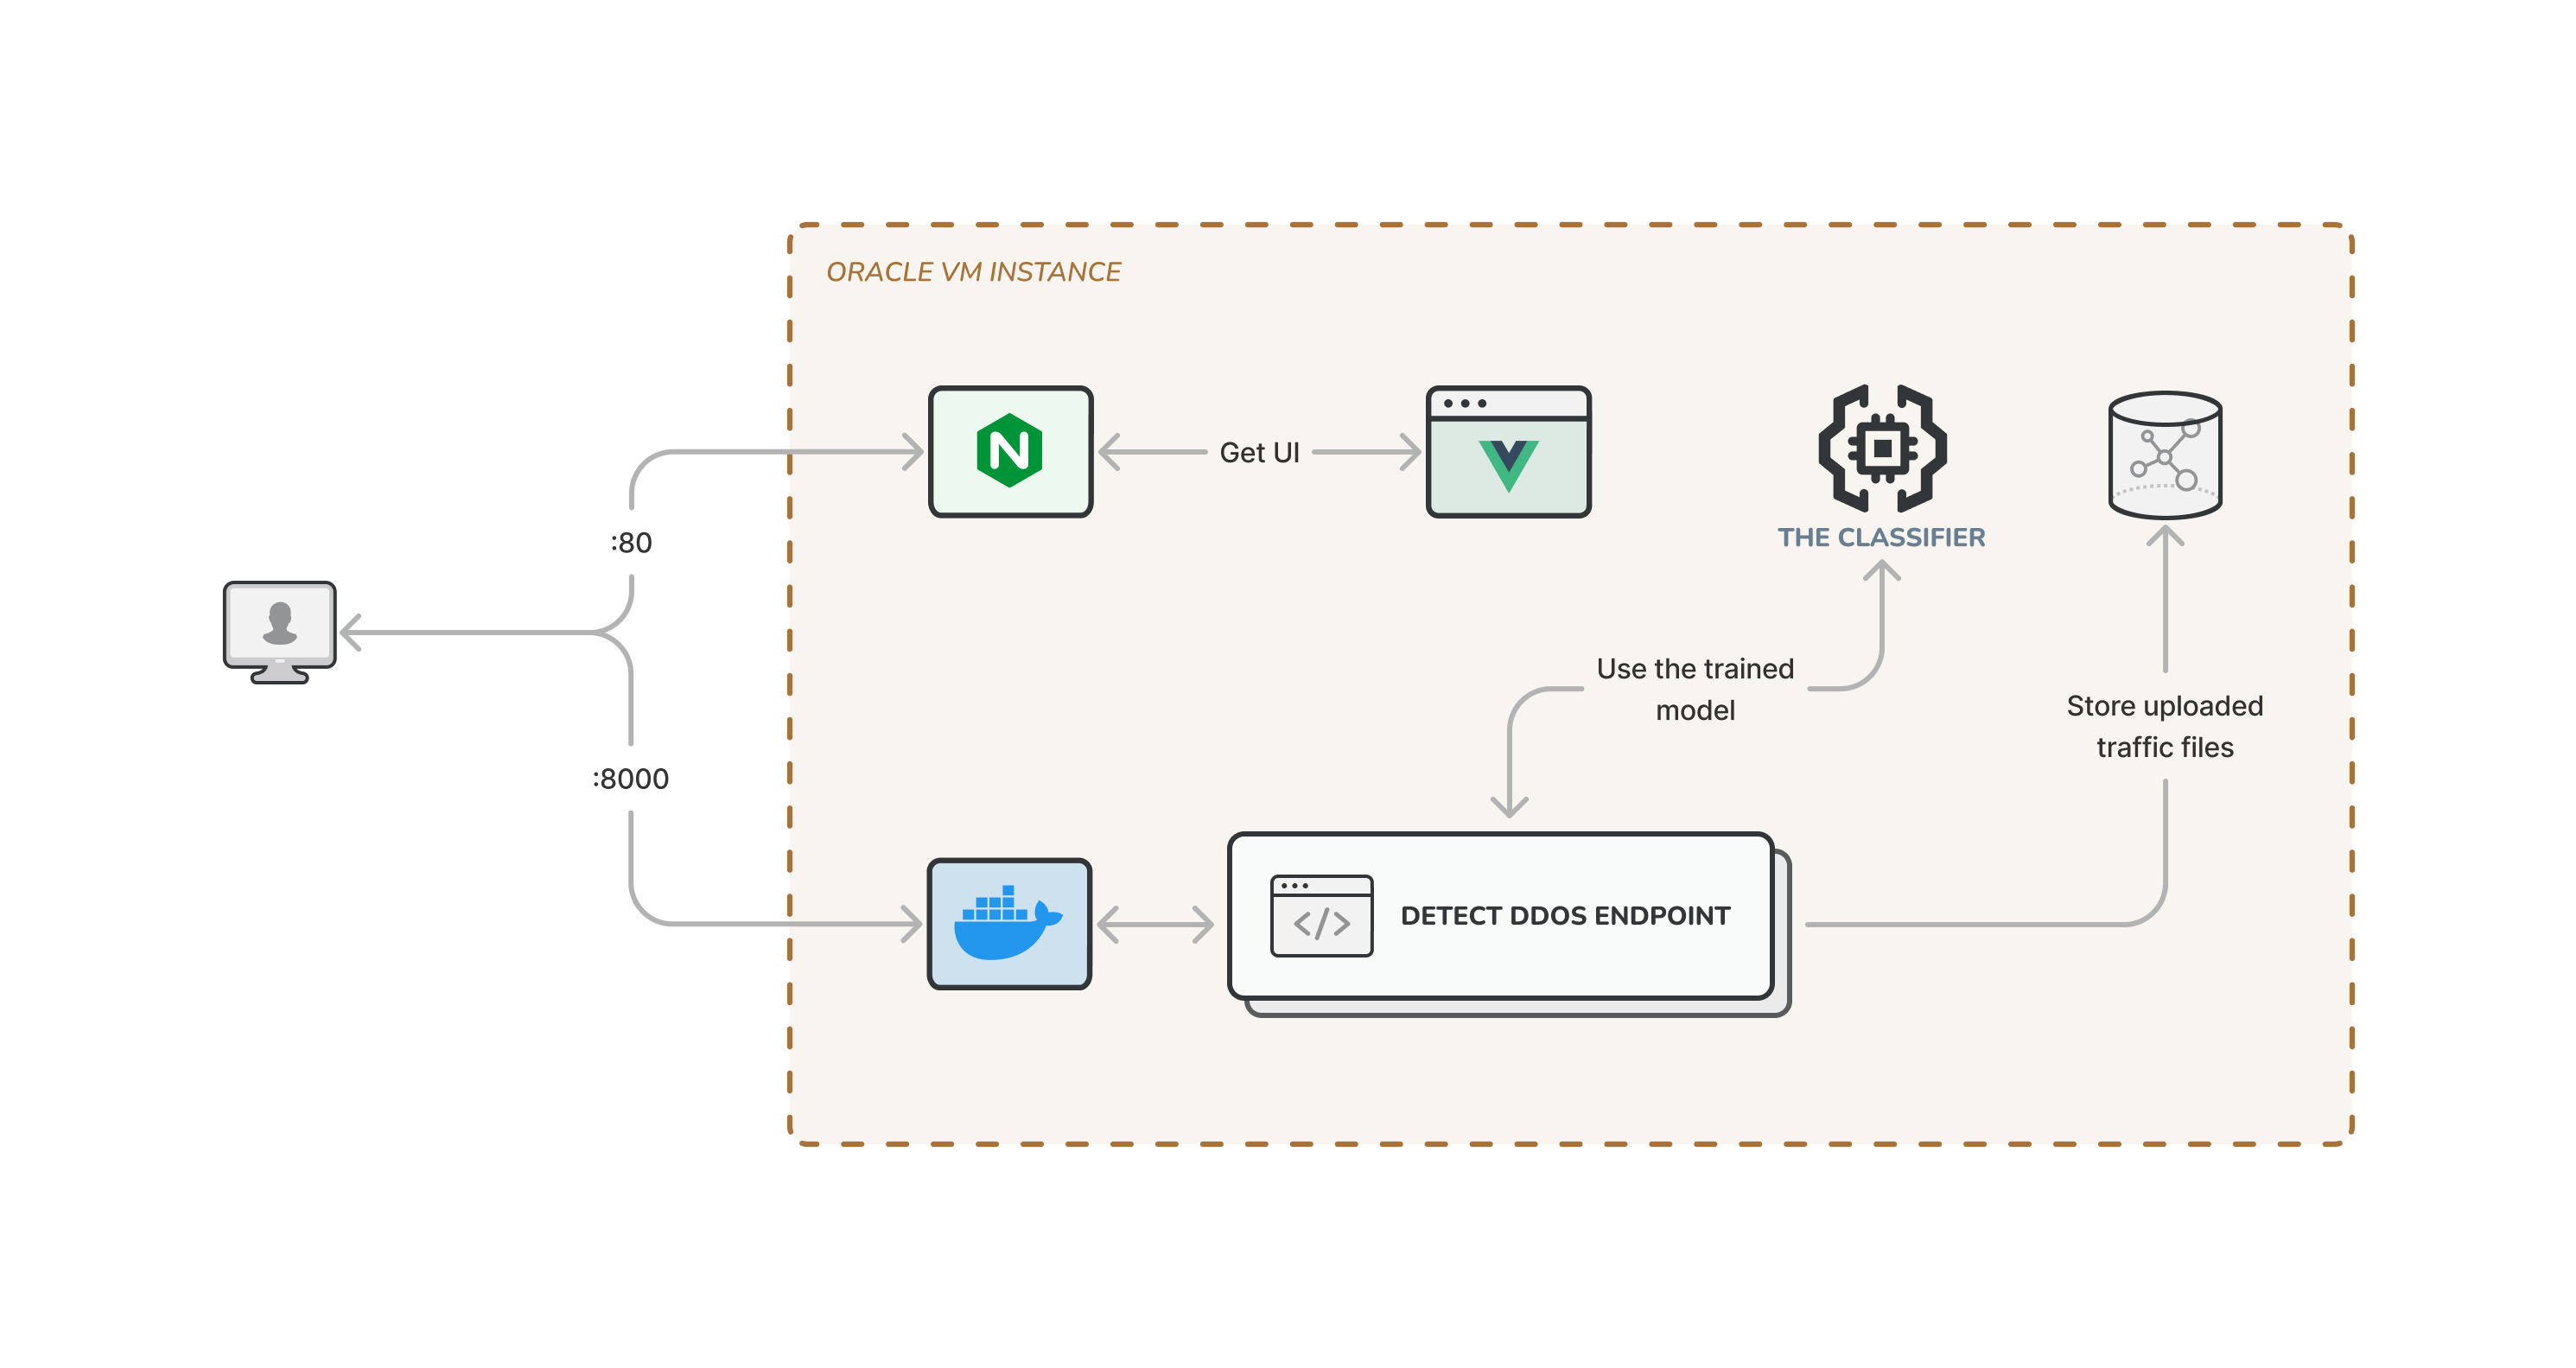
\includegraphics[width=1\textwidth]{./assets/images/architecture.png}
	\caption{Architecture of the application}
\end{figure}

The application architecture is designed to detect DDoS attacks from PCAP files. It consists of two main components: a \textbf{Vue.js} frontend application served by \textbf{Nginx} on port 80 and an API deployed using \textbf{Docker} on port 8000. The frontend provides a user interface for uploading PCAP files, while the API, built with \textbf{FastAPI}, processes these files to detect potential DDoS attacks.

The use of Docker for the API allows for easy deployment and scalability, as new instances of the API can be spun up quickly to handle increased traffic or processing demands. Overall, this architecture provides a scalable and efficient wrapper for our detecting DDoS attacks solution.

\clearpage

\section{Preview}
\begin{figure}[h]
	\centering
	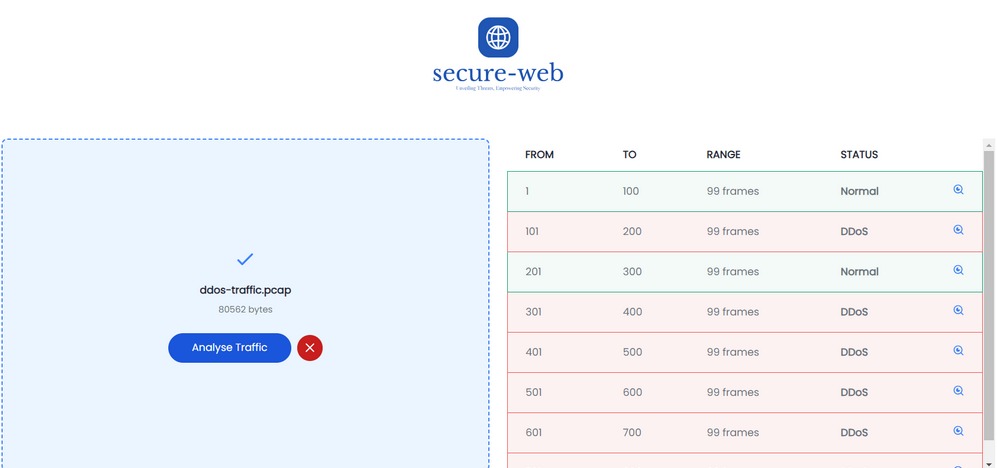
\includegraphics[width=1\textwidth]{./assets/images/preview.png}
	\caption{Preview of the application}
\end{figure} 